\documentclass[12pt, titlepage]{article}
\usepackage[USenglish]{babel}
\usepackage[utf8]{inputenc}
\usepackage{amssymb, amsmath}
\usepackage{bm}
\usepackage{color}
\usepackage[unicode]{hyperref}
\usepackage{url}
\hypersetup{
    colorlinks,
    citecolor=blue,
    filecolor=blue,
    linkcolor=blue,
    urlcolor=blue
}
\usepackage{graphicx}
\usepackage{grffile}
\usepackage{listings}
\usepackage{float}

\def\sgn{\operatorname{sgn}}
\title{LinUCB vs HybridLinUCB}
\date{\today}
\author{Radek Bartyzal}

\begin{document}
\begin{titlepage}
    \centering
    \vfill
    {\bfseries\Huge
        LinUCB vs HybridLinUCB in recommender systems
    }    
    \vfill
        
    
        
    {\bfseries\Large 
    Author:\\
    Radek Bartyzal (bartyrad@fit.cvut.cz)\\
    }    
    \vskip1cm
 
    \vskip1cm
    \today

    
    \vfill
\end{titlepage}

%\tableofcontents
\pagebreak

\section{Introduction}\label{sec:intro}
The algorithms LinUCB and HybridLinUCB are both introduced in the article A Contextual-Bandit Approach to
Personalized News Article Recommendation published in 2012.

The authors decided to model personalized recommendation of news
articles as a contextual bandit problem, a principled approach in
which a learning algorithm sequentially selects articles to serve
users based on contextual information about the users and articles,
while simultaneously adapting its article-selection strategy.

\section{Theory}\label{sec:theory}
Both algorithms are based on upper confidence bound algorithm (UCB) that uses a smarter way to balance
exploration and exploitation than a simple $\epsilon-greedy$ strategy. 
Specifically, in trial $t$, these algorithms
estimate both the mean payoff $\mu_{t,a}$ of each arm $a$ as well
as a corresponding confidence interval $c_{t,a}$, so that $|\mu_{t,a} - \mu_a| <
c_{t,a}$ holds with high probability. They then select the arm that
achieves a highest upper confidence bound: $a_t =
arg max_a (\mu_{t,a} + c_{t,a})$. With appropriately defined confidence intervals,
it can be shown that such algorithms have a small total $T$-
trial regret that is only logarithmic in the total number of trials $T$,
which turns out to be optimal. 

\subsection{LinUCB with Disjoint Linear Models (LinUCB)}
We assume the expected payoff of an arm $a$ is linear in its d-dimensional feature $x_{t,a}$ with some unknown coefficient vector $\theta^*_a$, namely:

$$
E[r_{t,a}|x_{t,a}] = x^T_{t,a}\theta^*_a
$$

\begin{itemize}
\item $a$ = arm = action = item to be recommended = e.g. article
\item $t$ = trial = in this case user ID
\item $r_{t,a}$ = reward of action $a$ in trial $t$ 
\item $x_{t,a}$ = features describing \textbf{both} user and the selected article $a$ at trial $t$. If the features of a user are his ratings, they will change with time.
\item $\theta^*_a$ = an unknown coefficient vector specific to arm $a$
\end{itemize}

This model is called disjoint since the parameters are not shared among different arms.
The solution is reached by a simple ridge regression and an algorithm allowing incremental updating of the parameter matrices can be seen in Figure \ref{fig:linUCB_alg}.

\begin{figure}[h]
 \centering
 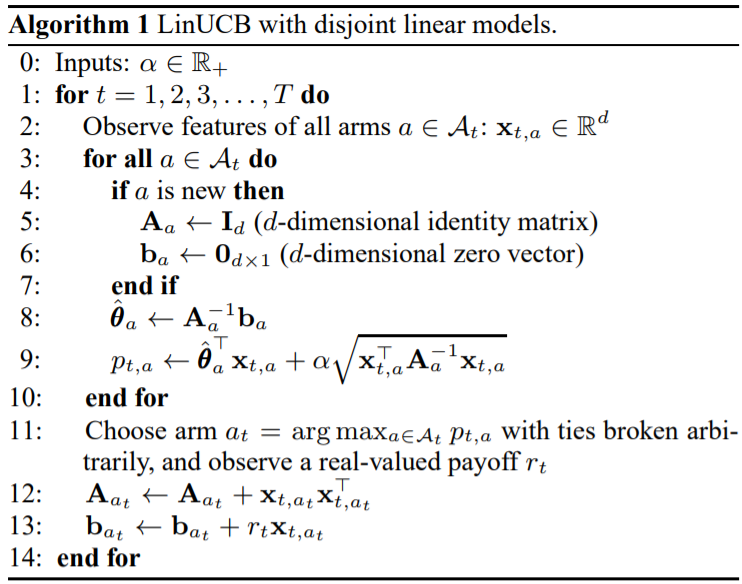
\includegraphics[scale=0.9]{img/LinUCB_alg}
 \caption{LinUCB algorithm with incrementally updating parameter matrices.\cite{cit:paper}}
 \label{fig:linUCB_alg}
\end{figure}

\subsection{LinUCB with Hybrid Linear Models (HybridLinUCB)}

In many applications, it is helpful to use features
that are shared by all arms, in addition to the arm-specific ones. For
example, in news article recommendation, a user may prefer only
articles about politics for which this provides a mechanism. Hence,
it is helpful to have features that have both shared and non-shared
components. Formally, we adopt the following hybrid model by
adding another linear term to the previous equation:

$$
E[r_{t,a}|x_{t,a}] = z^T_{t,a}\beta^* + x^T_{t,a}\theta^*_a 
$$

\begin{itemize}
\item $z_{t,a}$ = features of the current user/article combination
\item $\beta^*$ = an unknown coefficient vector common to all arms
\end{itemize}

The algorithm can be seen in Figure \ref{fig:HybridlinUCB_alg}.

\begin{figure}
 \centering
 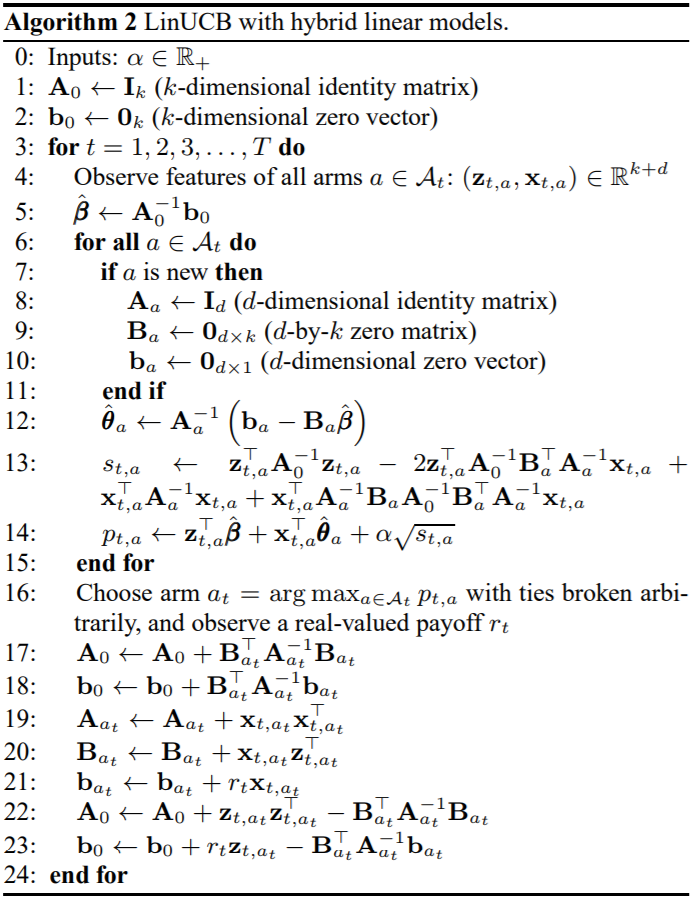
\includegraphics[scale=0.9]{img/HybridLinUCB_alg}
 \caption{HybridLinUCB algorithm with incrementally updating parameter matrices.\cite{cit:paper}}
 \label{fig:HybridlinUCB_alg}
\end{figure}


\section{Implementation}\label{sec:impl}
I have implemented both algorithms using the paper's notation for easy readability. The implementation does not support changing the arm set dynamically at the moment which leads to increased performance. The full project implementation can be found at \cite{cit:impl}.

Features in $x_{t,a}$ are a concatenation of features of user $t$ and item $a$ at the current time.

\begin{itemize}
\item user features = his ratings of all items = $R_u$
\item item features = movie genres = array of 1/0 describing whether the movie belongs to a genre. There are 19 genres.
\item $x_{t,a}$ = user features concatenated with item features
\item $z_{t,a}$ = only article features = genre vector
\end{itemize}

The algorithms are always run for a selected number of epochs.
An epoch means that the algorithm has iteratively generated a single recommendation for each user in the dataset. The ordering of the users is random in each epoch.


\section{Experiments}\label{sec:exp}

\subsection{Data preprocessing}
I have decided to use the MovieLens 100k dataset. 
It has 100 000 ratings, 1000 users and 1700 movies. \cite{cit:ml}

Due to the computational requirements I have taken a small subset of the whole dataset containing 100 items and 56 users. To ensure that all users have at least some ratings I have randomly added 3 ratings to each user.

As is customary in the recommendation world I have binarized the ratings from a scale of 1-5 to:

\begin{itemize}
\item 1 if the rating is 4 or larger = positive rating
\item -1 if the rating is smaller than 4 = negative rating
\item 0 = unknown rating
\end{itemize}

I have decided to keep the negative ratings separated from the unknown ones because I will need them to model the unknown user ratings.

\subsection{Modeling the user behavior}
The paper describes a sophisticated method to evaluate the algorithms offline which are interesting nevertheless such a procedure is out of scope of this project. Therefore I have decide to use a simple user model predicting a positive or negative rating of a yet unseen item.

Let item $a$ be recommended to user $u$.
If the user $u$ has already rated the item $a$, the returned reward will be 1 for positive rating or 0 for negative rating. Instead of these fixed values a Bernoulli distribution with high probability of 1/0 can be used to calculate the reward.

If the user $u$ has not rated the item $i$  yet the reward will be sampled from a Bernoulli distribution with $p$ equal to how much the user likes the genre of item $i$. Likability of a genre $g_a$ is calculated as a ratio of positive ratings of items belonging to genre $g_a$ to a number of negative ratings of items belonging to $g_a$. Only ratings by user $u$ are counted. If item $i$ belongs to multiple genres the resulting likability is calculated as an average of all the item $i$ genre likabilities.

\subsection{Fixed rewards}
In this experiment I have simply run the implemented algorithm with settings described in the previous chapters for 50 epochs. The results can be seen in Figures \ref{fig:linUCB-100it} and \ref{fig:HybridlinUCB-100it}. 


\begin{figure}[h!]
 \centering
 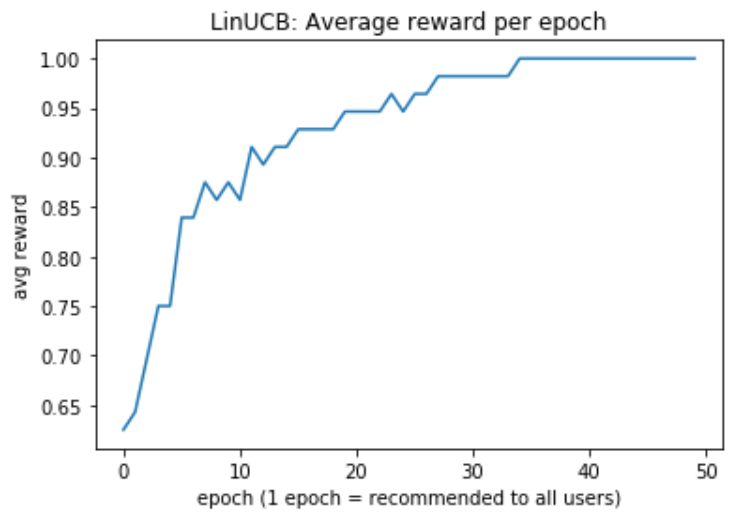
\includegraphics[scale=0.5]{img/LinUCB-100items-50epochs}
 \caption{LinUCB trained on 100 items and 56 users for 50 epochs.}
 \label{fig:linUCB-100it}
\end{figure}

\begin{figure}[h!]
 \centering
 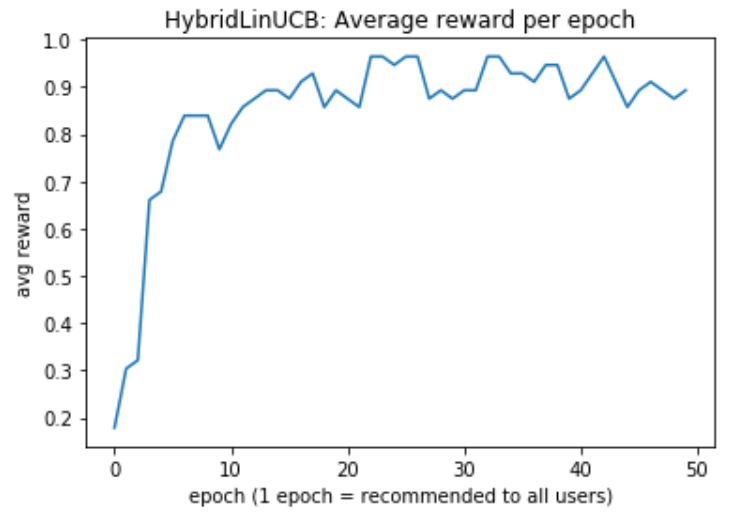
\includegraphics[scale=0.5]{img/HybridLinUCB-100items-50epochs}
 \caption{HybridLinUCB trained on 100 items and 56 users for 50 epochs. }
 \label{fig:HybridlinUCB-100it}
\end{figure}



\section{Conclusion}\label{sec:conclusion}


\begin{thebibliography}{0}

  \bibitem[1]{cit:paper} Li, Lihong, et al. "A contextual-bandit approach to personalized news article recommendation." Proceedings of the 19th international conference on World wide web. ACM, 2010. Accessible from: \url{https://arxiv.org/abs/1003.0146}
  
  \bibitem[2]{cit:impl} Project implementation at: \url{https://github.com/BartyzalRadek/contextual-bandits-recommender}
  
  \bibitem[3]{cit:ml} F. Maxwell Harper and Joseph A. Konstan. 2015. The MovieLens Datasets:
History and Context. ACM Transactions on Interactive Intelligent
Systems (TiiS) 5, 4, Article 19 (December 2015), 19 pages.
DOI=http://dx.doi.org/10.1145/2827872 Accessible from: \url{https://grouplens.org/datasets/movielens/100k/}



\end{thebibliography}


\end{document}